% ============================================================
%  paper_figures.tex — TikZ architecture diagrams
%  Paper 3 — Constraint-Aware Ordering for Directed Traceability
%  ÉTS PhD / ACM Distributed Ledger Technologies, Autumn 2026
%
%  Compile standalone:
%    pdflatex paper_figures.tex
%
%  Or include individual figures in the main paper:
%    % ============================================================
%  paper_figures.tex — TikZ architecture diagrams
%  Paper 3 — Constraint-Aware Ordering for Directed Traceability
%  ÉTS PhD / ACM Distributed Ledger Technologies, Autumn 2026
%
%  Compile standalone:
%    pdflatex paper_figures.tex
%
%  Or include individual figures in the main paper:
%    % ============================================================
%  paper_figures.tex — TikZ architecture diagrams
%  Paper 3 — Constraint-Aware Ordering for Directed Traceability
%  ÉTS PhD / ACM Distributed Ledger Technologies, Autumn 2026
%
%  Compile standalone:
%    pdflatex paper_figures.tex
%
%  Or include individual figures in the main paper:
%    % ============================================================
%  paper_figures.tex — TikZ architecture diagrams
%  Paper 3 — Constraint-Aware Ordering for Directed Traceability
%  ÉTS PhD / ACM Distributed Ledger Technologies, Autumn 2026
%
%  Compile standalone:
%    pdflatex paper_figures.tex
%
%  Or include individual figures in the main paper:
%    \input{paper_figures.tex}   % loads \figArchitectures, \figCache
%    ...
%    \figArchitectures
%    \figCache
% ============================================================

\documentclass[tikz, border=4pt]{standalone}

\usepackage{tikz}
\usepackage{xcolor}
\usepackage{amsmath}
\usepackage{amssymb}
\usepackage{helvet}          % sans-serif labels
\renewcommand{\familydefault}{\sfdefault}

\usetikzlibrary{
  arrows.meta,
  backgrounds,
  calc,
  decorations.pathreplacing,
  fit,
  positioning,
  shapes.geometric,
  shapes.multipart,
}

% ── Colour palette (colourblind-safe) ──────────────────────────────────────────
\definecolor{cML}{RGB}{72, 120, 207}       % blue  — M_L
\definecolor{cEndo}{RGB}{214,  95,  95}    % red   — M_D endo
\definecolor{cExo}{RGB}{ 90, 180,  90}     % green — M_D exo
\definecolor{cBlock}{RGB}{245,245,245}     % light grey block fill
\definecolor{cBorder}{RGB}{180,180,180}    % border grey
\definecolor{cReject}{RGB}{220, 80, 80}    % rejection red
\definecolor{cCommit}{RGB}{ 60,160, 60}    % commit green
\definecolor{cSpec}{RGB}{255,200,100}      % speculative amber
\definecolor{cStable}{RGB}{100,180,240}    % stable blue

% ── Common TikZ styles ─────────────────────────────────────────────────────────
\tikzset{
  % Generic box
  box/.style={
    rectangle, rounded corners=3pt,
    draw=#1!70!black, fill=#1!12,
    minimum width=2.8cm, minimum height=0.55cm,
    font=\small\sffamily, align=center,
    inner sep=4pt,
  },
  % Arrow
  arr/.style={-{Stealth[length=5pt]}, thick},
  arrdashed/.style={-{Stealth[length=5pt]}, thick, dashed},
  % Column header
  colhead/.style={
    font=\small\bfseries\sffamily,
    minimum width=3.2cm, align=center,
  },
  % Column frame
  colframe/.style={
    rectangle, rounded corners=5pt,
    draw=#1!50!black, fill=#1!6,
    inner sep=8pt,
  },
  % Reject label
  reject/.style={font=\tiny\sffamily, color=cReject},
  % Annotation brace label
  bracelab/.style={font=\scriptsize\sffamily, midway},
}

% ==============================================================================
%  FIGURE 1 — Three-architecture comparison
% ==============================================================================
\newcommand{\figArchitectures}{%
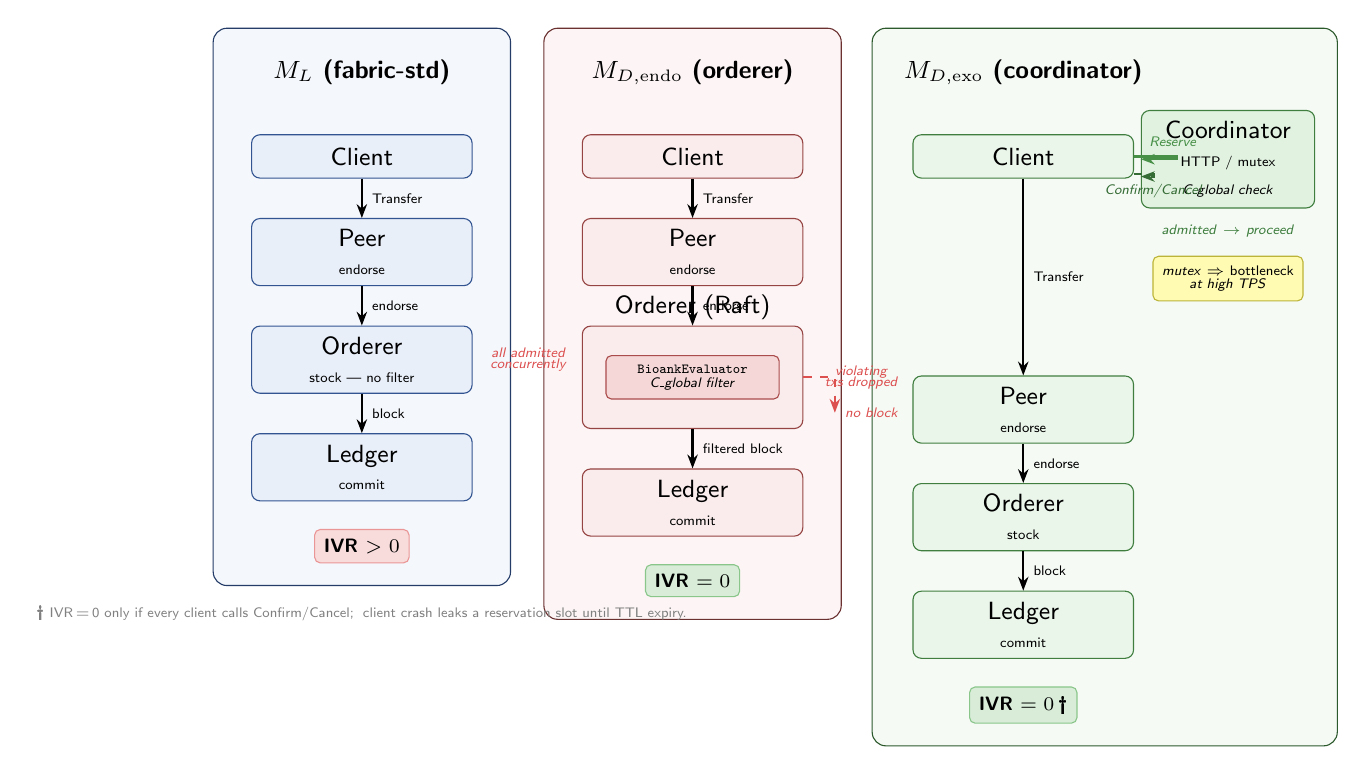
\begin{tikzpicture}[node distance=0.38cm]

% ── Column spacing ─────────────────────────────────────────────────────────────
\def\colA{0}
\def\colB{4.2}
\def\colC{8.4}

% ══════════════════════════════════════════════════════════
%  M_L column
% ══════════════════════════════════════════════════════════
\begin{scope}[xshift=\colA cm]
  % Header
  \node[colhead] (hML) at (1.6, 0)
    {$M_L$ \textbf{(fabric-std)}};

  % Nodes
  \node[box=cML, below=0.5cm of hML]     (cliML)  {Client};
  \node[box=cML, below=0.5cm of cliML]   (peerML) {Peer\\[-1pt]{\tiny endorse}};
  \node[box=cML, below=0.5cm of peerML]  (ordML)  {Orderer\\[-1pt]{\tiny stock — no filter}};
  \node[box=cML, below=0.5cm of ordML]   (ledML)  {Ledger\\[-1pt]{\tiny commit}};

  % Arrows
  \draw[arr] (cliML)  -- node[right, font=\tiny]{Transfer} (peerML);
  \draw[arr] (peerML) -- node[right, font=\tiny]{endorse}  (ordML);
  \draw[arr] (ordML)  -- node[right, font=\tiny]{block}    (ledML);

  % IVR badge
  \node[
    rectangle, rounded corners=2pt,
    fill=cReject!20, draw=cReject!60,
    font=\scriptsize\sffamily\bfseries,
    below=0.35cm of ledML,
  ] (ivrML) {IVR $> 0$};

  % Annotation: concurrent envelopes all admitted
  \node[
    font=\tiny\sffamily, text=cReject, align=center,
    right=0.1cm of ordML,
  ] {\textit{all admitted}\\[-2pt]\textit{concurrently}};

  % Column frame
  \begin{pgfonlayer}{background}
    \node[colframe=cML,
      fit=(hML)(cliML)(peerML)(ordML)(ledML)(ivrML),
    ] {};
  \end{pgfonlayer}
\end{scope}

% ══════════════════════════════════════════════════════════
%  M_D endogenous column
% ══════════════════════════════════════════════════════════
\begin{scope}[xshift=\colB cm]
  % Header
  \node[colhead] (hEndo) at (1.6, 0)
    {$M_{D,\mathrm{endo}}$ \textbf{(orderer)}};

  % Nodes
  \node[box=cEndo, below=0.5cm of hEndo]    (cliEndo)  {Client};
  \node[box=cEndo, below=0.5cm of cliEndo]  (peerEndo) {Peer\\[-1pt]{\tiny endorse}};

  % Orderer with evaluator sub-box
  \node[
    rectangle, rounded corners=3pt,
    draw=cEndo!70!black, fill=cEndo!12,
    minimum width=2.8cm, minimum height=1.3cm,
    below=0.5cm of peerEndo,
    font=\small\sffamily, align=center,
    inner sep=4pt,
  ] (ordEndo) {};
  \node[font=\small\sffamily, above=-0.05cm] at (ordEndo.north) {Orderer (Raft)};
  \node[
    rectangle, rounded corners=2pt,
    draw=cEndo!80!black, fill=cEndo!25,
    minimum width=2.2cm, minimum height=0.42cm,
    font=\tiny\sffamily, align=center,
  ] at (ordEndo.center) (eval) {\texttt{BioankEvaluator}\\[-1pt]\textit{C\_global filter}};

  \node[box=cEndo, below=0.5cm of ordEndo]  (ledEndo) {Ledger\\[-1pt]{\tiny commit}};

  % Drop path
  \node[
    font=\tiny\sffamily, text=cReject, align=center,
    right=0.15cm of ordEndo,
  ] (drop) {\textit{violating}\\[-2pt]\textit{txs dropped}};
  \draw[arrdashed, color=cReject]
    (ordEndo.east) -- ++(0.4,0) -- ++(0,-0.45)
    node[right, font=\tiny\sffamily, text=cReject]{\textit{no block}};

  % Main arrows
  \draw[arr] (cliEndo)  -- node[right, font=\tiny]{Transfer} (peerEndo);
  \draw[arr] (peerEndo) -- node[right, font=\tiny]{endorse}  (ordEndo);
  \draw[arr] (ordEndo)  -- node[right, font=\tiny]{filtered block} (ledEndo);

  % IVR badge
  \node[
    rectangle, rounded corners=2pt,
    fill=cCommit!20, draw=cCommit!60,
    font=\scriptsize\sffamily\bfseries,
    below=0.35cm of ledEndo,
  ] (ivrEndo) {IVR $= 0$};

  % Column frame
  \begin{pgfonlayer}{background}
    \node[colframe=cEndo,
      fit=(hEndo)(cliEndo)(peerEndo)(ordEndo)(ledEndo)(ivrEndo),
    ] {};
  \end{pgfonlayer}
\end{scope}

% ══════════════════════════════════════════════════════════
%  M_D exogenous column
% ══════════════════════════════════════════════════════════
\begin{scope}[xshift=\colC cm]
  % Header
  \node[colhead] (hExo) at (1.6, 0)
    {$M_{D,\mathrm{exo}}$ \textbf{(coordinator)}};

  % Coordinator (off to the right of main flow)
  \node[
    rectangle, rounded corners=3pt,
    draw=cExo!70!black, fill=cExo!18,
    minimum width=2.2cm, minimum height=0.9cm,
    font=\small\sffamily, align=center,
    inner sep=4pt,
  ] (coord) at (4.2, -1.1) {Coordinator\\[-1pt]{\tiny HTTP / mutex}\\[-1pt]{\tiny \textit{C\_global check}}};

  % Main flow nodes
  \node[box=cExo, below=0.5cm of hExo]    (cliExo)  {Client};
  \node[box=cExo, below=2.5cm of cliExo]  (peerExo) {Peer\\[-1pt]{\tiny endorse}};
  \node[box=cExo, below=0.5cm of peerExo] (ordExo)  {Orderer\\[-1pt]{\tiny stock}};
  \node[box=cExo, below=0.5cm of ordExo]  (ledExo)  {Ledger\\[-1pt]{\tiny commit}};

  % Reserve arrow (client → coordinator)
  \draw[arr, color=cExo!80!black]
    (cliExo.east) -- ++(0.55,0)
    node[above, font=\tiny\sffamily, pos=0.9]{\textit{Reserve}}
    |- (coord.west);

  % Confirm/Cancel arrow (client → coordinator)
  \draw[arrdashed, color=cExo!60!black]
    ($(cliExo.east)+(0.0,-0.22)$) -- ++(0.25,0)
    |- ($(coord.west)+(0,-0.22)$)
    node[below, font=\tiny\sffamily, pos=0.1]{\textit{Confirm/Cancel}};

  % Coordinator → admitted label
  \node[
    font=\tiny\sffamily, text=cExo!70!black,
    below=0.08cm of coord,
  ] {\textit{admitted} $\rightarrow$ \textit{proceed}};

  % Main arrows
  \draw[arr] (cliExo)  -- node[right, font=\tiny]{Transfer} (peerExo);
  \draw[arr] (peerExo) -- node[right, font=\tiny]{endorse}  (ordExo);
  \draw[arr] (ordExo)  -- node[right, font=\tiny]{block}    (ledExo);

  % Bottleneck annotation
  \node[
    rectangle, rounded corners=2pt,
    fill=yellow!30, draw=yellow!70!black,
    font=\tiny\sffamily, align=center,
    below=0.1cm of coord,
  ] at ($(coord.south)+(0,-0.5)$) {\textit{mutex} $\Rightarrow$ bottleneck\\[-1pt]\textit{at high TPS}};

  % IVR badge
  \node[
    rectangle, rounded corners=2pt,
    fill=cCommit!20, draw=cCommit!60,
    font=\scriptsize\sffamily\bfseries,
    below=0.35cm of ledExo,
  ] (ivrExo) {IVR $= 0$\,†};

  % Column frame
  \begin{pgfonlayer}{background}
    \node[colframe=cExo,
      fit=(hExo)(cliExo)(coord)(peerExo)(ordExo)(ledExo)(ivrExo),
    ] {};
  \end{pgfonlayer}
\end{scope}

% ── Global caption note ────────────────────────────────────────────────────────
\node[
  font=\tiny\sffamily, text=gray, align=left,
  below=1.2cm of ledML,
] {† IVR\,$=$\,0 only if every client calls Confirm/Cancel;\; client crash leaks a reservation slot until TTL expiry.};

\end{tikzpicture}
}% end \figArchitectures


% ==============================================================================
%  FIGURE 2 — Stable / speculative cache lifecycle
% ==============================================================================
\newcommand{\figCache}{%
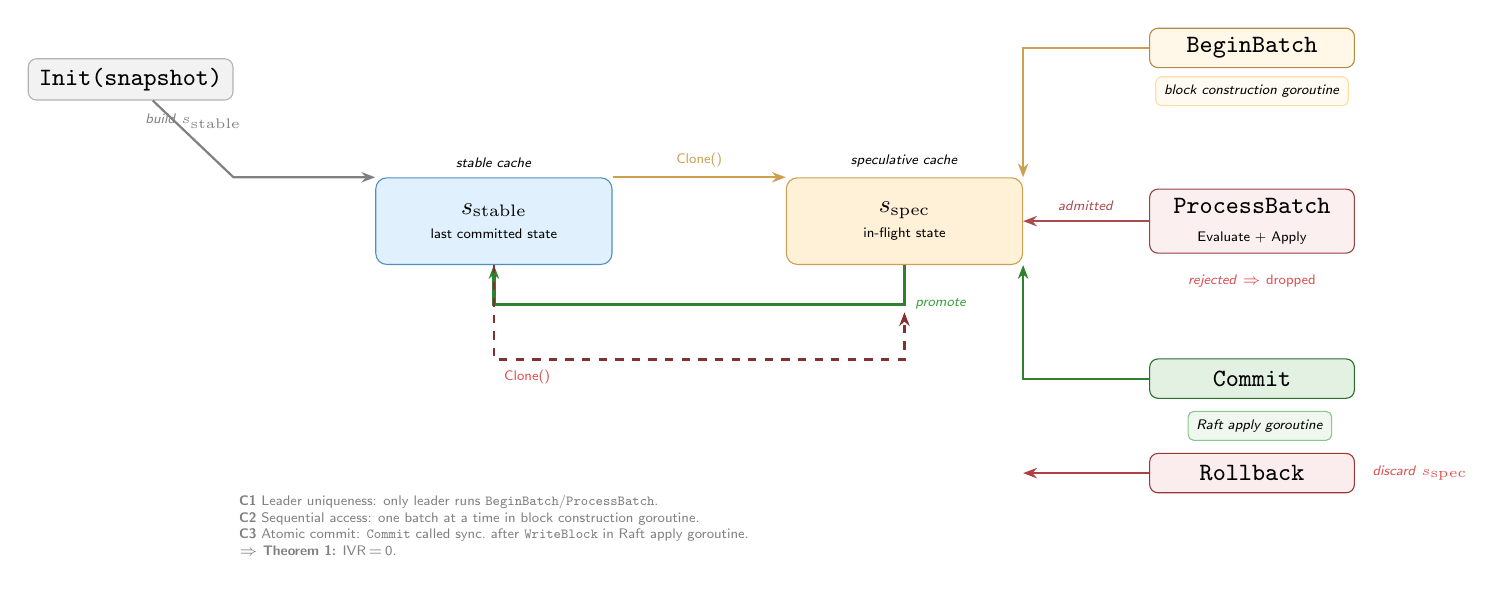
\begin{tikzpicture}[
  node distance=0.5cm and 1.8cm,
]

% ── Cache pair display ─────────────────────────────────────────────────────────
\def\cacheW{3.0cm}
\def\cacheH{1.1cm}

% Stable state box
\node[
  rectangle, rounded corners=4pt,
  draw=cStable!80!black, fill=cStable!20,
  minimum width=\cacheW, minimum height=\cacheH,
  font=\small\sffamily, align=center,
  label={[font=\tiny\sffamily]above:\textit{stable cache}},
] (stable) at (0,0) {$s_{\mathrm{stable}}$\\[-2pt]{\tiny last committed state}};

% Speculative state box
\node[
  rectangle, rounded corners=4pt,
  draw=cSpec!80!black, fill=cSpec!25,
  minimum width=\cacheW, minimum height=\cacheH,
  font=\small\sffamily, align=center,
  label={[font=\tiny\sffamily]above:\textit{speculative cache}},
  right=2.2cm of stable,
] (spec) {$s_{\mathrm{spec}}$\\[-2pt]{\tiny in-flight state}};

% ── Events on the left ─────────────────────────────────────────────────────────

% HandleChain / Init
\node[
  rectangle, rounded corners=3pt,
  draw=gray!60, fill=gray!10,
  minimum width=2.6cm, minimum height=0.5cm,
  font=\small\sffamily, align=center,
  left=1.8cm of stable, yshift=1.8cm,
] (init) {\texttt{Init(snapshot)}};

\draw[arr, gray]
  (init) -- node[above, font=\tiny\sffamily]{\textit{build} $s_{\mathrm{stable}}$}
  (stable.north -| init.east) -- (stable.north west);

% ── Events on the right (block construction loop) ─────────────────────────────

% BeginBatch
\node[
  rectangle, rounded corners=3pt,
  draw=cSpec!70!black, fill=cSpec!15,
  minimum width=2.6cm, minimum height=0.5cm,
  font=\small\sffamily, align=center,
  right=1.6cm of spec, yshift=2.2cm,
] (begin) {\texttt{BeginBatch}};

\draw[arr, color=cSpec!80!black]
  (stable.north east) --
  node[above, font=\tiny\sffamily]{Clone()} (spec.north west);
\draw[arr, color=cSpec!80!black]
  (begin) -- (spec.north east |- begin) -- (spec.north east);

% ProcessBatch — envelope loop
\node[
  rectangle, rounded corners=3pt,
  draw=cEndo!70!black, fill=cEndo!10,
  minimum width=2.6cm, minimum height=0.75cm,
  font=\small\sffamily, align=center,
  right=1.6cm of spec,
] (proc) {\texttt{ProcessBatch}\\[-1pt]{\tiny Evaluate + Apply}};

\draw[arr, color=cEndo!80!black]
  (proc.west) -- node[above, font=\tiny\sffamily]{\textit{admitted}} (spec.east);

% Rejected envelope
\node[
  font=\tiny\sffamily, text=cReject, align=center,
  below=0.15cm of proc,
] (rej) {\textit{rejected} $\Rightarrow$ dropped};

% Commit (success path)
\node[
  rectangle, rounded corners=3pt,
  draw=cCommit!70!black, fill=cCommit!15,
  minimum width=2.6cm, minimum height=0.5cm,
  font=\small\sffamily, align=center,
  right=1.6cm of spec, yshift=-2.0cm,
] (commit) {\texttt{Commit}};

\draw[arr, color=cCommit!80!black]
  (commit.west) -- (spec.east |- commit) -- (spec.south east);
\draw[arr, color=cCommit!80!black, very thick]
  (spec.south) -- ++(0,-0.5)
  node[right, font=\tiny\sffamily, text=cCommit]{\textit{promote}}
  -| (stable.south);

% Rollback (failure path)
\node[
  rectangle, rounded corners=3pt,
  draw=cReject!70!black, fill=cReject!10,
  minimum width=2.6cm, minimum height=0.5cm,
  font=\small\sffamily, align=center,
  right=1.6cm of spec, yshift=-3.2cm,
] (rollback) {\texttt{Rollback}};

\draw[arr, color=cReject!80!black]
  (rollback.west) -- (spec.east |- rollback);
\node[font=\tiny\sffamily, text=cReject, right=0.1cm of rollback]
  {\textit{discard} $s_{\mathrm{spec}}$};

% Stable re-clone on rollback
\draw[arrdashed, color=cReject!60!black]
  (stable.south) -- ++(0,-1.2)
  node[below right, font=\tiny\sffamily, text=cReject]{Clone()}
  -| ($(spec.south)+(0,-0.6)$);

% ── Goroutine labels ───────────────────────────────────────────────────────────
\node[
  rectangle, rounded corners=2pt,
  draw=cSpec!60, fill=cSpec!8,
  font=\tiny\sffamily, align=center, inner sep=3pt,
] at ($(begin)!0.5!(proc) + (0, 0.55)$) {\textit{block construction goroutine}};

\node[
  rectangle, rounded corners=2pt,
  draw=cCommit!60, fill=cCommit!8,
  font=\tiny\sffamily, align=center, inner sep=3pt,
] at ($(commit)!0.5!(rollback) + (0.1, 0)$) {\textit{Raft apply goroutine}};

% ── Invariant annotations ─────────────────────────────────────────────────────
\node[
  font=\tiny\sffamily, text=gray, align=left,
  below=2.8cm of stable,
] {
  \textbf{C1} Leader uniqueness: only leader runs \texttt{BeginBatch}/\texttt{ProcessBatch}.\\
  \textbf{C2} Sequential access: one batch at a time in block construction goroutine.\\
  \textbf{C3} Atomic commit: \texttt{Commit} called sync.\ after \texttt{WriteBlock} in Raft apply goroutine.\\
  $\Rightarrow$ \textbf{Theorem 1:} IVR\,$=$\,0.
};

\end{tikzpicture}
}% end \figCache


% ==============================================================================
%  Render both figures as standalone pages
% ==============================================================================
\begin{document}

% Page 1 — Architecture comparison
\figArchitectures

\newpage

% Page 2 — Cache lifecycle
\figCache

\end{document}
   % loads \figArchitectures, \figCache
%    ...
%    \figArchitectures
%    \figCache
% ============================================================

\documentclass[tikz, border=4pt]{standalone}

\usepackage{tikz}
\usepackage{xcolor}
\usepackage{amsmath}
\usepackage{amssymb}
\usepackage{helvet}          % sans-serif labels
\renewcommand{\familydefault}{\sfdefault}

\usetikzlibrary{
  arrows.meta,
  backgrounds,
  calc,
  decorations.pathreplacing,
  fit,
  positioning,
  shapes.geometric,
  shapes.multipart,
}

% ── Colour palette (colourblind-safe) ──────────────────────────────────────────
\definecolor{cML}{RGB}{72, 120, 207}       % blue  — M_L
\definecolor{cEndo}{RGB}{214,  95,  95}    % red   — M_D endo
\definecolor{cExo}{RGB}{ 90, 180,  90}     % green — M_D exo
\definecolor{cBlock}{RGB}{245,245,245}     % light grey block fill
\definecolor{cBorder}{RGB}{180,180,180}    % border grey
\definecolor{cReject}{RGB}{220, 80, 80}    % rejection red
\definecolor{cCommit}{RGB}{ 60,160, 60}    % commit green
\definecolor{cSpec}{RGB}{255,200,100}      % speculative amber
\definecolor{cStable}{RGB}{100,180,240}    % stable blue

% ── Common TikZ styles ─────────────────────────────────────────────────────────
\tikzset{
  % Generic box
  box/.style={
    rectangle, rounded corners=3pt,
    draw=#1!70!black, fill=#1!12,
    minimum width=2.8cm, minimum height=0.55cm,
    font=\small\sffamily, align=center,
    inner sep=4pt,
  },
  % Arrow
  arr/.style={-{Stealth[length=5pt]}, thick},
  arrdashed/.style={-{Stealth[length=5pt]}, thick, dashed},
  % Column header
  colhead/.style={
    font=\small\bfseries\sffamily,
    minimum width=3.2cm, align=center,
  },
  % Column frame
  colframe/.style={
    rectangle, rounded corners=5pt,
    draw=#1!50!black, fill=#1!6,
    inner sep=8pt,
  },
  % Reject label
  reject/.style={font=\tiny\sffamily, color=cReject},
  % Annotation brace label
  bracelab/.style={font=\scriptsize\sffamily, midway},
}

% ==============================================================================
%  FIGURE 1 — Three-architecture comparison
% ==============================================================================
\newcommand{\figArchitectures}{%
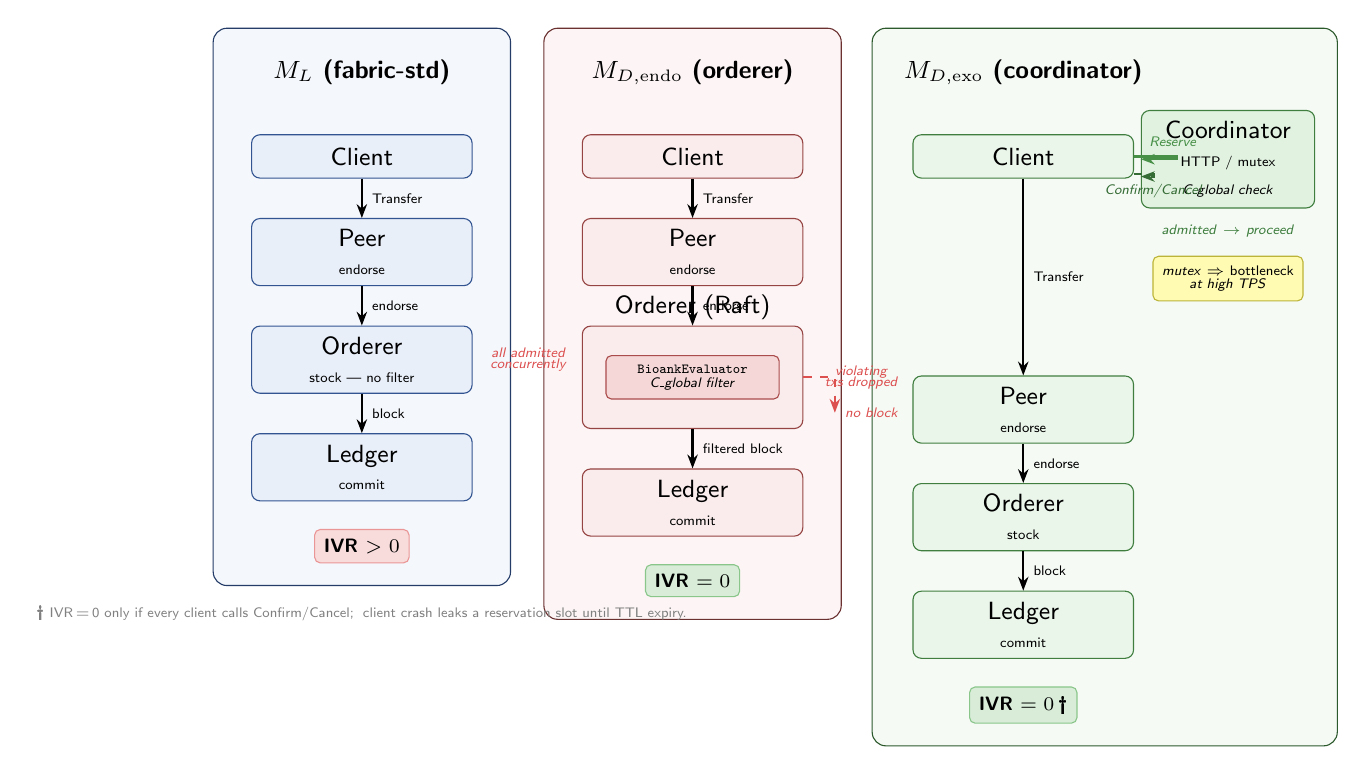
\begin{tikzpicture}[node distance=0.38cm]

% ── Column spacing ─────────────────────────────────────────────────────────────
\def\colA{0}
\def\colB{4.2}
\def\colC{8.4}

% ══════════════════════════════════════════════════════════
%  M_L column
% ══════════════════════════════════════════════════════════
\begin{scope}[xshift=\colA cm]
  % Header
  \node[colhead] (hML) at (1.6, 0)
    {$M_L$ \textbf{(fabric-std)}};

  % Nodes
  \node[box=cML, below=0.5cm of hML]     (cliML)  {Client};
  \node[box=cML, below=0.5cm of cliML]   (peerML) {Peer\\[-1pt]{\tiny endorse}};
  \node[box=cML, below=0.5cm of peerML]  (ordML)  {Orderer\\[-1pt]{\tiny stock — no filter}};
  \node[box=cML, below=0.5cm of ordML]   (ledML)  {Ledger\\[-1pt]{\tiny commit}};

  % Arrows
  \draw[arr] (cliML)  -- node[right, font=\tiny]{Transfer} (peerML);
  \draw[arr] (peerML) -- node[right, font=\tiny]{endorse}  (ordML);
  \draw[arr] (ordML)  -- node[right, font=\tiny]{block}    (ledML);

  % IVR badge
  \node[
    rectangle, rounded corners=2pt,
    fill=cReject!20, draw=cReject!60,
    font=\scriptsize\sffamily\bfseries,
    below=0.35cm of ledML,
  ] (ivrML) {IVR $> 0$};

  % Annotation: concurrent envelopes all admitted
  \node[
    font=\tiny\sffamily, text=cReject, align=center,
    right=0.1cm of ordML,
  ] {\textit{all admitted}\\[-2pt]\textit{concurrently}};

  % Column frame
  \begin{pgfonlayer}{background}
    \node[colframe=cML,
      fit=(hML)(cliML)(peerML)(ordML)(ledML)(ivrML),
    ] {};
  \end{pgfonlayer}
\end{scope}

% ══════════════════════════════════════════════════════════
%  M_D endogenous column
% ══════════════════════════════════════════════════════════
\begin{scope}[xshift=\colB cm]
  % Header
  \node[colhead] (hEndo) at (1.6, 0)
    {$M_{D,\mathrm{endo}}$ \textbf{(orderer)}};

  % Nodes
  \node[box=cEndo, below=0.5cm of hEndo]    (cliEndo)  {Client};
  \node[box=cEndo, below=0.5cm of cliEndo]  (peerEndo) {Peer\\[-1pt]{\tiny endorse}};

  % Orderer with evaluator sub-box
  \node[
    rectangle, rounded corners=3pt,
    draw=cEndo!70!black, fill=cEndo!12,
    minimum width=2.8cm, minimum height=1.3cm,
    below=0.5cm of peerEndo,
    font=\small\sffamily, align=center,
    inner sep=4pt,
  ] (ordEndo) {};
  \node[font=\small\sffamily, above=-0.05cm] at (ordEndo.north) {Orderer (Raft)};
  \node[
    rectangle, rounded corners=2pt,
    draw=cEndo!80!black, fill=cEndo!25,
    minimum width=2.2cm, minimum height=0.42cm,
    font=\tiny\sffamily, align=center,
  ] at (ordEndo.center) (eval) {\texttt{BioankEvaluator}\\[-1pt]\textit{C\_global filter}};

  \node[box=cEndo, below=0.5cm of ordEndo]  (ledEndo) {Ledger\\[-1pt]{\tiny commit}};

  % Drop path
  \node[
    font=\tiny\sffamily, text=cReject, align=center,
    right=0.15cm of ordEndo,
  ] (drop) {\textit{violating}\\[-2pt]\textit{txs dropped}};
  \draw[arrdashed, color=cReject]
    (ordEndo.east) -- ++(0.4,0) -- ++(0,-0.45)
    node[right, font=\tiny\sffamily, text=cReject]{\textit{no block}};

  % Main arrows
  \draw[arr] (cliEndo)  -- node[right, font=\tiny]{Transfer} (peerEndo);
  \draw[arr] (peerEndo) -- node[right, font=\tiny]{endorse}  (ordEndo);
  \draw[arr] (ordEndo)  -- node[right, font=\tiny]{filtered block} (ledEndo);

  % IVR badge
  \node[
    rectangle, rounded corners=2pt,
    fill=cCommit!20, draw=cCommit!60,
    font=\scriptsize\sffamily\bfseries,
    below=0.35cm of ledEndo,
  ] (ivrEndo) {IVR $= 0$};

  % Column frame
  \begin{pgfonlayer}{background}
    \node[colframe=cEndo,
      fit=(hEndo)(cliEndo)(peerEndo)(ordEndo)(ledEndo)(ivrEndo),
    ] {};
  \end{pgfonlayer}
\end{scope}

% ══════════════════════════════════════════════════════════
%  M_D exogenous column
% ══════════════════════════════════════════════════════════
\begin{scope}[xshift=\colC cm]
  % Header
  \node[colhead] (hExo) at (1.6, 0)
    {$M_{D,\mathrm{exo}}$ \textbf{(coordinator)}};

  % Coordinator (off to the right of main flow)
  \node[
    rectangle, rounded corners=3pt,
    draw=cExo!70!black, fill=cExo!18,
    minimum width=2.2cm, minimum height=0.9cm,
    font=\small\sffamily, align=center,
    inner sep=4pt,
  ] (coord) at (4.2, -1.1) {Coordinator\\[-1pt]{\tiny HTTP / mutex}\\[-1pt]{\tiny \textit{C\_global check}}};

  % Main flow nodes
  \node[box=cExo, below=0.5cm of hExo]    (cliExo)  {Client};
  \node[box=cExo, below=2.5cm of cliExo]  (peerExo) {Peer\\[-1pt]{\tiny endorse}};
  \node[box=cExo, below=0.5cm of peerExo] (ordExo)  {Orderer\\[-1pt]{\tiny stock}};
  \node[box=cExo, below=0.5cm of ordExo]  (ledExo)  {Ledger\\[-1pt]{\tiny commit}};

  % Reserve arrow (client → coordinator)
  \draw[arr, color=cExo!80!black]
    (cliExo.east) -- ++(0.55,0)
    node[above, font=\tiny\sffamily, pos=0.9]{\textit{Reserve}}
    |- (coord.west);

  % Confirm/Cancel arrow (client → coordinator)
  \draw[arrdashed, color=cExo!60!black]
    ($(cliExo.east)+(0.0,-0.22)$) -- ++(0.25,0)
    |- ($(coord.west)+(0,-0.22)$)
    node[below, font=\tiny\sffamily, pos=0.1]{\textit{Confirm/Cancel}};

  % Coordinator → admitted label
  \node[
    font=\tiny\sffamily, text=cExo!70!black,
    below=0.08cm of coord,
  ] {\textit{admitted} $\rightarrow$ \textit{proceed}};

  % Main arrows
  \draw[arr] (cliExo)  -- node[right, font=\tiny]{Transfer} (peerExo);
  \draw[arr] (peerExo) -- node[right, font=\tiny]{endorse}  (ordExo);
  \draw[arr] (ordExo)  -- node[right, font=\tiny]{block}    (ledExo);

  % Bottleneck annotation
  \node[
    rectangle, rounded corners=2pt,
    fill=yellow!30, draw=yellow!70!black,
    font=\tiny\sffamily, align=center,
    below=0.1cm of coord,
  ] at ($(coord.south)+(0,-0.5)$) {\textit{mutex} $\Rightarrow$ bottleneck\\[-1pt]\textit{at high TPS}};

  % IVR badge
  \node[
    rectangle, rounded corners=2pt,
    fill=cCommit!20, draw=cCommit!60,
    font=\scriptsize\sffamily\bfseries,
    below=0.35cm of ledExo,
  ] (ivrExo) {IVR $= 0$\,†};

  % Column frame
  \begin{pgfonlayer}{background}
    \node[colframe=cExo,
      fit=(hExo)(cliExo)(coord)(peerExo)(ordExo)(ledExo)(ivrExo),
    ] {};
  \end{pgfonlayer}
\end{scope}

% ── Global caption note ────────────────────────────────────────────────────────
\node[
  font=\tiny\sffamily, text=gray, align=left,
  below=1.2cm of ledML,
] {† IVR\,$=$\,0 only if every client calls Confirm/Cancel;\; client crash leaks a reservation slot until TTL expiry.};

\end{tikzpicture}
}% end \figArchitectures


% ==============================================================================
%  FIGURE 2 — Stable / speculative cache lifecycle
% ==============================================================================
\newcommand{\figCache}{%
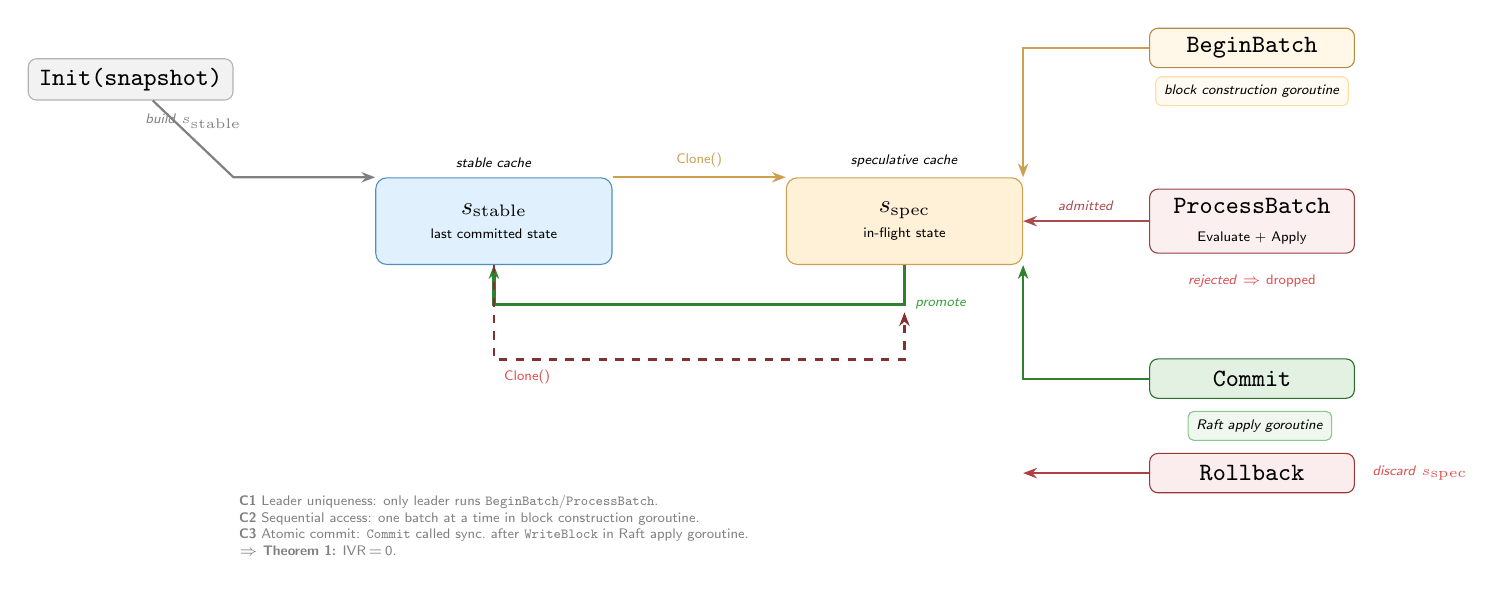
\begin{tikzpicture}[
  node distance=0.5cm and 1.8cm,
]

% ── Cache pair display ─────────────────────────────────────────────────────────
\def\cacheW{3.0cm}
\def\cacheH{1.1cm}

% Stable state box
\node[
  rectangle, rounded corners=4pt,
  draw=cStable!80!black, fill=cStable!20,
  minimum width=\cacheW, minimum height=\cacheH,
  font=\small\sffamily, align=center,
  label={[font=\tiny\sffamily]above:\textit{stable cache}},
] (stable) at (0,0) {$s_{\mathrm{stable}}$\\[-2pt]{\tiny last committed state}};

% Speculative state box
\node[
  rectangle, rounded corners=4pt,
  draw=cSpec!80!black, fill=cSpec!25,
  minimum width=\cacheW, minimum height=\cacheH,
  font=\small\sffamily, align=center,
  label={[font=\tiny\sffamily]above:\textit{speculative cache}},
  right=2.2cm of stable,
] (spec) {$s_{\mathrm{spec}}$\\[-2pt]{\tiny in-flight state}};

% ── Events on the left ─────────────────────────────────────────────────────────

% HandleChain / Init
\node[
  rectangle, rounded corners=3pt,
  draw=gray!60, fill=gray!10,
  minimum width=2.6cm, minimum height=0.5cm,
  font=\small\sffamily, align=center,
  left=1.8cm of stable, yshift=1.8cm,
] (init) {\texttt{Init(snapshot)}};

\draw[arr, gray]
  (init) -- node[above, font=\tiny\sffamily]{\textit{build} $s_{\mathrm{stable}}$}
  (stable.north -| init.east) -- (stable.north west);

% ── Events on the right (block construction loop) ─────────────────────────────

% BeginBatch
\node[
  rectangle, rounded corners=3pt,
  draw=cSpec!70!black, fill=cSpec!15,
  minimum width=2.6cm, minimum height=0.5cm,
  font=\small\sffamily, align=center,
  right=1.6cm of spec, yshift=2.2cm,
] (begin) {\texttt{BeginBatch}};

\draw[arr, color=cSpec!80!black]
  (stable.north east) --
  node[above, font=\tiny\sffamily]{Clone()} (spec.north west);
\draw[arr, color=cSpec!80!black]
  (begin) -- (spec.north east |- begin) -- (spec.north east);

% ProcessBatch — envelope loop
\node[
  rectangle, rounded corners=3pt,
  draw=cEndo!70!black, fill=cEndo!10,
  minimum width=2.6cm, minimum height=0.75cm,
  font=\small\sffamily, align=center,
  right=1.6cm of spec,
] (proc) {\texttt{ProcessBatch}\\[-1pt]{\tiny Evaluate + Apply}};

\draw[arr, color=cEndo!80!black]
  (proc.west) -- node[above, font=\tiny\sffamily]{\textit{admitted}} (spec.east);

% Rejected envelope
\node[
  font=\tiny\sffamily, text=cReject, align=center,
  below=0.15cm of proc,
] (rej) {\textit{rejected} $\Rightarrow$ dropped};

% Commit (success path)
\node[
  rectangle, rounded corners=3pt,
  draw=cCommit!70!black, fill=cCommit!15,
  minimum width=2.6cm, minimum height=0.5cm,
  font=\small\sffamily, align=center,
  right=1.6cm of spec, yshift=-2.0cm,
] (commit) {\texttt{Commit}};

\draw[arr, color=cCommit!80!black]
  (commit.west) -- (spec.east |- commit) -- (spec.south east);
\draw[arr, color=cCommit!80!black, very thick]
  (spec.south) -- ++(0,-0.5)
  node[right, font=\tiny\sffamily, text=cCommit]{\textit{promote}}
  -| (stable.south);

% Rollback (failure path)
\node[
  rectangle, rounded corners=3pt,
  draw=cReject!70!black, fill=cReject!10,
  minimum width=2.6cm, minimum height=0.5cm,
  font=\small\sffamily, align=center,
  right=1.6cm of spec, yshift=-3.2cm,
] (rollback) {\texttt{Rollback}};

\draw[arr, color=cReject!80!black]
  (rollback.west) -- (spec.east |- rollback);
\node[font=\tiny\sffamily, text=cReject, right=0.1cm of rollback]
  {\textit{discard} $s_{\mathrm{spec}}$};

% Stable re-clone on rollback
\draw[arrdashed, color=cReject!60!black]
  (stable.south) -- ++(0,-1.2)
  node[below right, font=\tiny\sffamily, text=cReject]{Clone()}
  -| ($(spec.south)+(0,-0.6)$);

% ── Goroutine labels ───────────────────────────────────────────────────────────
\node[
  rectangle, rounded corners=2pt,
  draw=cSpec!60, fill=cSpec!8,
  font=\tiny\sffamily, align=center, inner sep=3pt,
] at ($(begin)!0.5!(proc) + (0, 0.55)$) {\textit{block construction goroutine}};

\node[
  rectangle, rounded corners=2pt,
  draw=cCommit!60, fill=cCommit!8,
  font=\tiny\sffamily, align=center, inner sep=3pt,
] at ($(commit)!0.5!(rollback) + (0.1, 0)$) {\textit{Raft apply goroutine}};

% ── Invariant annotations ─────────────────────────────────────────────────────
\node[
  font=\tiny\sffamily, text=gray, align=left,
  below=2.8cm of stable,
] {
  \textbf{C1} Leader uniqueness: only leader runs \texttt{BeginBatch}/\texttt{ProcessBatch}.\\
  \textbf{C2} Sequential access: one batch at a time in block construction goroutine.\\
  \textbf{C3} Atomic commit: \texttt{Commit} called sync.\ after \texttt{WriteBlock} in Raft apply goroutine.\\
  $\Rightarrow$ \textbf{Theorem 1:} IVR\,$=$\,0.
};

\end{tikzpicture}
}% end \figCache


% ==============================================================================
%  Render both figures as standalone pages
% ==============================================================================
\begin{document}

% Page 1 — Architecture comparison
\figArchitectures

\newpage

% Page 2 — Cache lifecycle
\figCache

\end{document}
   % loads \figArchitectures, \figCache
%    ...
%    \figArchitectures
%    \figCache
% ============================================================

\documentclass[tikz, border=4pt]{standalone}

\usepackage{tikz}
\usepackage{xcolor}
\usepackage{amsmath}
\usepackage{amssymb}
\usepackage{helvet}          % sans-serif labels
\renewcommand{\familydefault}{\sfdefault}

\usetikzlibrary{
  arrows.meta,
  backgrounds,
  calc,
  decorations.pathreplacing,
  fit,
  positioning,
  shapes.geometric,
  shapes.multipart,
}

% ── Colour palette (colourblind-safe) ──────────────────────────────────────────
\definecolor{cML}{RGB}{72, 120, 207}       % blue  — M_L
\definecolor{cEndo}{RGB}{214,  95,  95}    % red   — M_D endo
\definecolor{cExo}{RGB}{ 90, 180,  90}     % green — M_D exo
\definecolor{cBlock}{RGB}{245,245,245}     % light grey block fill
\definecolor{cBorder}{RGB}{180,180,180}    % border grey
\definecolor{cReject}{RGB}{220, 80, 80}    % rejection red
\definecolor{cCommit}{RGB}{ 60,160, 60}    % commit green
\definecolor{cSpec}{RGB}{255,200,100}      % speculative amber
\definecolor{cStable}{RGB}{100,180,240}    % stable blue

% ── Common TikZ styles ─────────────────────────────────────────────────────────
\tikzset{
  % Generic box
  box/.style={
    rectangle, rounded corners=3pt,
    draw=#1!70!black, fill=#1!12,
    minimum width=2.8cm, minimum height=0.55cm,
    font=\small\sffamily, align=center,
    inner sep=4pt,
  },
  % Arrow
  arr/.style={-{Stealth[length=5pt]}, thick},
  arrdashed/.style={-{Stealth[length=5pt]}, thick, dashed},
  % Column header
  colhead/.style={
    font=\small\bfseries\sffamily,
    minimum width=3.2cm, align=center,
  },
  % Column frame
  colframe/.style={
    rectangle, rounded corners=5pt,
    draw=#1!50!black, fill=#1!6,
    inner sep=8pt,
  },
  % Reject label
  reject/.style={font=\tiny\sffamily, color=cReject},
  % Annotation brace label
  bracelab/.style={font=\scriptsize\sffamily, midway},
}

% ==============================================================================
%  FIGURE 1 — Three-architecture comparison
% ==============================================================================
\newcommand{\figArchitectures}{%
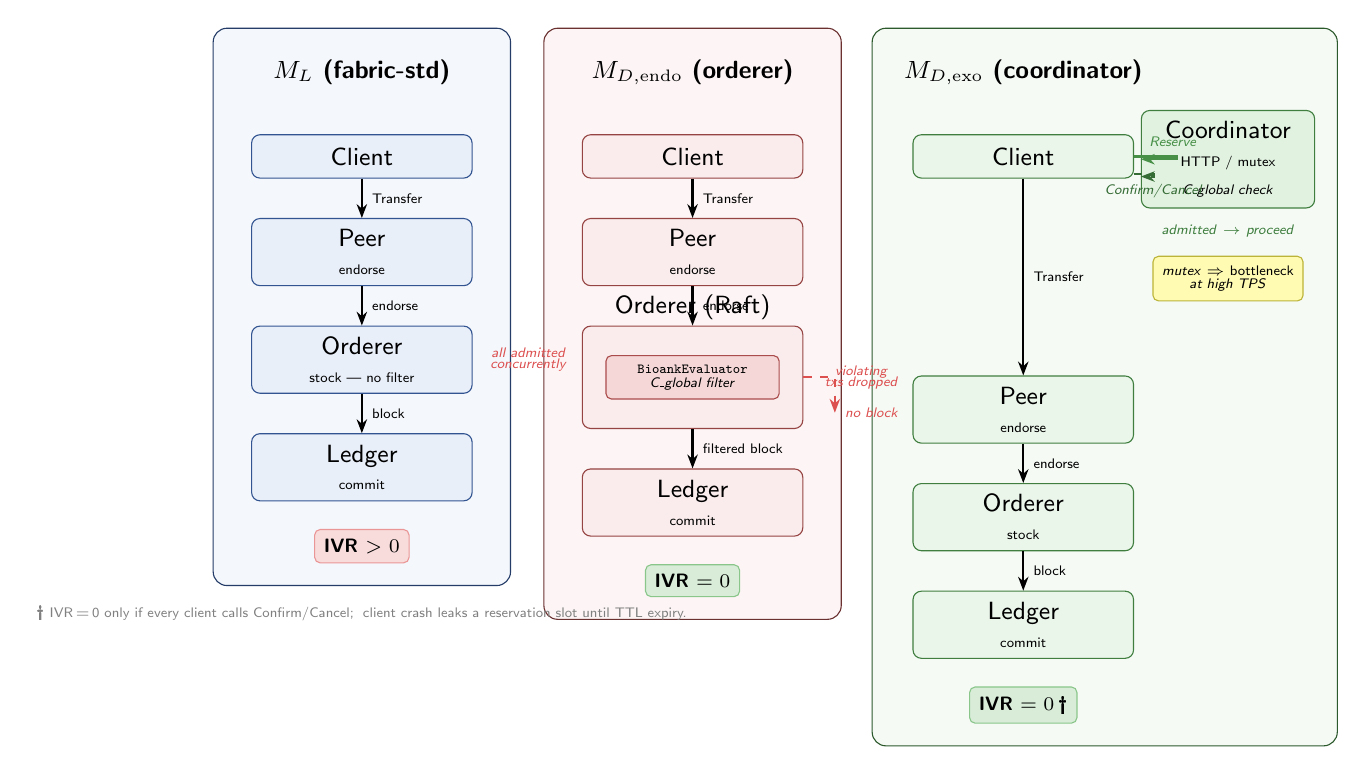
\begin{tikzpicture}[node distance=0.38cm]

% ── Column spacing ─────────────────────────────────────────────────────────────
\def\colA{0}
\def\colB{4.2}
\def\colC{8.4}

% ══════════════════════════════════════════════════════════
%  M_L column
% ══════════════════════════════════════════════════════════
\begin{scope}[xshift=\colA cm]
  % Header
  \node[colhead] (hML) at (1.6, 0)
    {$M_L$ \textbf{(fabric-std)}};

  % Nodes
  \node[box=cML, below=0.5cm of hML]     (cliML)  {Client};
  \node[box=cML, below=0.5cm of cliML]   (peerML) {Peer\\[-1pt]{\tiny endorse}};
  \node[box=cML, below=0.5cm of peerML]  (ordML)  {Orderer\\[-1pt]{\tiny stock — no filter}};
  \node[box=cML, below=0.5cm of ordML]   (ledML)  {Ledger\\[-1pt]{\tiny commit}};

  % Arrows
  \draw[arr] (cliML)  -- node[right, font=\tiny]{Transfer} (peerML);
  \draw[arr] (peerML) -- node[right, font=\tiny]{endorse}  (ordML);
  \draw[arr] (ordML)  -- node[right, font=\tiny]{block}    (ledML);

  % IVR badge
  \node[
    rectangle, rounded corners=2pt,
    fill=cReject!20, draw=cReject!60,
    font=\scriptsize\sffamily\bfseries,
    below=0.35cm of ledML,
  ] (ivrML) {IVR $> 0$};

  % Annotation: concurrent envelopes all admitted
  \node[
    font=\tiny\sffamily, text=cReject, align=center,
    right=0.1cm of ordML,
  ] {\textit{all admitted}\\[-2pt]\textit{concurrently}};

  % Column frame
  \begin{pgfonlayer}{background}
    \node[colframe=cML,
      fit=(hML)(cliML)(peerML)(ordML)(ledML)(ivrML),
    ] {};
  \end{pgfonlayer}
\end{scope}

% ══════════════════════════════════════════════════════════
%  M_D endogenous column
% ══════════════════════════════════════════════════════════
\begin{scope}[xshift=\colB cm]
  % Header
  \node[colhead] (hEndo) at (1.6, 0)
    {$M_{D,\mathrm{endo}}$ \textbf{(orderer)}};

  % Nodes
  \node[box=cEndo, below=0.5cm of hEndo]    (cliEndo)  {Client};
  \node[box=cEndo, below=0.5cm of cliEndo]  (peerEndo) {Peer\\[-1pt]{\tiny endorse}};

  % Orderer with evaluator sub-box
  \node[
    rectangle, rounded corners=3pt,
    draw=cEndo!70!black, fill=cEndo!12,
    minimum width=2.8cm, minimum height=1.3cm,
    below=0.5cm of peerEndo,
    font=\small\sffamily, align=center,
    inner sep=4pt,
  ] (ordEndo) {};
  \node[font=\small\sffamily, above=-0.05cm] at (ordEndo.north) {Orderer (Raft)};
  \node[
    rectangle, rounded corners=2pt,
    draw=cEndo!80!black, fill=cEndo!25,
    minimum width=2.2cm, minimum height=0.42cm,
    font=\tiny\sffamily, align=center,
  ] at (ordEndo.center) (eval) {\texttt{BioankEvaluator}\\[-1pt]\textit{C\_global filter}};

  \node[box=cEndo, below=0.5cm of ordEndo]  (ledEndo) {Ledger\\[-1pt]{\tiny commit}};

  % Drop path
  \node[
    font=\tiny\sffamily, text=cReject, align=center,
    right=0.15cm of ordEndo,
  ] (drop) {\textit{violating}\\[-2pt]\textit{txs dropped}};
  \draw[arrdashed, color=cReject]
    (ordEndo.east) -- ++(0.4,0) -- ++(0,-0.45)
    node[right, font=\tiny\sffamily, text=cReject]{\textit{no block}};

  % Main arrows
  \draw[arr] (cliEndo)  -- node[right, font=\tiny]{Transfer} (peerEndo);
  \draw[arr] (peerEndo) -- node[right, font=\tiny]{endorse}  (ordEndo);
  \draw[arr] (ordEndo)  -- node[right, font=\tiny]{filtered block} (ledEndo);

  % IVR badge
  \node[
    rectangle, rounded corners=2pt,
    fill=cCommit!20, draw=cCommit!60,
    font=\scriptsize\sffamily\bfseries,
    below=0.35cm of ledEndo,
  ] (ivrEndo) {IVR $= 0$};

  % Column frame
  \begin{pgfonlayer}{background}
    \node[colframe=cEndo,
      fit=(hEndo)(cliEndo)(peerEndo)(ordEndo)(ledEndo)(ivrEndo),
    ] {};
  \end{pgfonlayer}
\end{scope}

% ══════════════════════════════════════════════════════════
%  M_D exogenous column
% ══════════════════════════════════════════════════════════
\begin{scope}[xshift=\colC cm]
  % Header
  \node[colhead] (hExo) at (1.6, 0)
    {$M_{D,\mathrm{exo}}$ \textbf{(coordinator)}};

  % Coordinator (off to the right of main flow)
  \node[
    rectangle, rounded corners=3pt,
    draw=cExo!70!black, fill=cExo!18,
    minimum width=2.2cm, minimum height=0.9cm,
    font=\small\sffamily, align=center,
    inner sep=4pt,
  ] (coord) at (4.2, -1.1) {Coordinator\\[-1pt]{\tiny HTTP / mutex}\\[-1pt]{\tiny \textit{C\_global check}}};

  % Main flow nodes
  \node[box=cExo, below=0.5cm of hExo]    (cliExo)  {Client};
  \node[box=cExo, below=2.5cm of cliExo]  (peerExo) {Peer\\[-1pt]{\tiny endorse}};
  \node[box=cExo, below=0.5cm of peerExo] (ordExo)  {Orderer\\[-1pt]{\tiny stock}};
  \node[box=cExo, below=0.5cm of ordExo]  (ledExo)  {Ledger\\[-1pt]{\tiny commit}};

  % Reserve arrow (client → coordinator)
  \draw[arr, color=cExo!80!black]
    (cliExo.east) -- ++(0.55,0)
    node[above, font=\tiny\sffamily, pos=0.9]{\textit{Reserve}}
    |- (coord.west);

  % Confirm/Cancel arrow (client → coordinator)
  \draw[arrdashed, color=cExo!60!black]
    ($(cliExo.east)+(0.0,-0.22)$) -- ++(0.25,0)
    |- ($(coord.west)+(0,-0.22)$)
    node[below, font=\tiny\sffamily, pos=0.1]{\textit{Confirm/Cancel}};

  % Coordinator → admitted label
  \node[
    font=\tiny\sffamily, text=cExo!70!black,
    below=0.08cm of coord,
  ] {\textit{admitted} $\rightarrow$ \textit{proceed}};

  % Main arrows
  \draw[arr] (cliExo)  -- node[right, font=\tiny]{Transfer} (peerExo);
  \draw[arr] (peerExo) -- node[right, font=\tiny]{endorse}  (ordExo);
  \draw[arr] (ordExo)  -- node[right, font=\tiny]{block}    (ledExo);

  % Bottleneck annotation
  \node[
    rectangle, rounded corners=2pt,
    fill=yellow!30, draw=yellow!70!black,
    font=\tiny\sffamily, align=center,
    below=0.1cm of coord,
  ] at ($(coord.south)+(0,-0.5)$) {\textit{mutex} $\Rightarrow$ bottleneck\\[-1pt]\textit{at high TPS}};

  % IVR badge
  \node[
    rectangle, rounded corners=2pt,
    fill=cCommit!20, draw=cCommit!60,
    font=\scriptsize\sffamily\bfseries,
    below=0.35cm of ledExo,
  ] (ivrExo) {IVR $= 0$\,†};

  % Column frame
  \begin{pgfonlayer}{background}
    \node[colframe=cExo,
      fit=(hExo)(cliExo)(coord)(peerExo)(ordExo)(ledExo)(ivrExo),
    ] {};
  \end{pgfonlayer}
\end{scope}

% ── Global caption note ────────────────────────────────────────────────────────
\node[
  font=\tiny\sffamily, text=gray, align=left,
  below=1.2cm of ledML,
] {† IVR\,$=$\,0 only if every client calls Confirm/Cancel;\; client crash leaks a reservation slot until TTL expiry.};

\end{tikzpicture}
}% end \figArchitectures


% ==============================================================================
%  FIGURE 2 — Stable / speculative cache lifecycle
% ==============================================================================
\newcommand{\figCache}{%
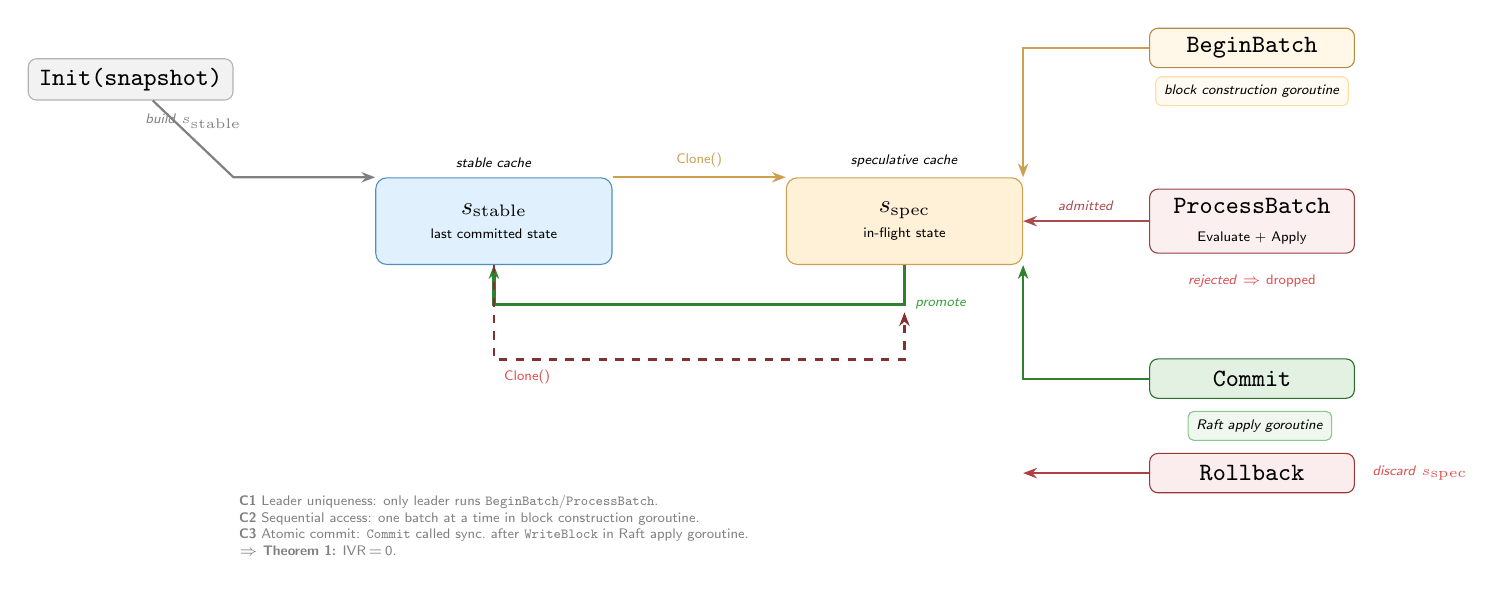
\begin{tikzpicture}[
  node distance=0.5cm and 1.8cm,
]

% ── Cache pair display ─────────────────────────────────────────────────────────
\def\cacheW{3.0cm}
\def\cacheH{1.1cm}

% Stable state box
\node[
  rectangle, rounded corners=4pt,
  draw=cStable!80!black, fill=cStable!20,
  minimum width=\cacheW, minimum height=\cacheH,
  font=\small\sffamily, align=center,
  label={[font=\tiny\sffamily]above:\textit{stable cache}},
] (stable) at (0,0) {$s_{\mathrm{stable}}$\\[-2pt]{\tiny last committed state}};

% Speculative state box
\node[
  rectangle, rounded corners=4pt,
  draw=cSpec!80!black, fill=cSpec!25,
  minimum width=\cacheW, minimum height=\cacheH,
  font=\small\sffamily, align=center,
  label={[font=\tiny\sffamily]above:\textit{speculative cache}},
  right=2.2cm of stable,
] (spec) {$s_{\mathrm{spec}}$\\[-2pt]{\tiny in-flight state}};

% ── Events on the left ─────────────────────────────────────────────────────────

% HandleChain / Init
\node[
  rectangle, rounded corners=3pt,
  draw=gray!60, fill=gray!10,
  minimum width=2.6cm, minimum height=0.5cm,
  font=\small\sffamily, align=center,
  left=1.8cm of stable, yshift=1.8cm,
] (init) {\texttt{Init(snapshot)}};

\draw[arr, gray]
  (init) -- node[above, font=\tiny\sffamily]{\textit{build} $s_{\mathrm{stable}}$}
  (stable.north -| init.east) -- (stable.north west);

% ── Events on the right (block construction loop) ─────────────────────────────

% BeginBatch
\node[
  rectangle, rounded corners=3pt,
  draw=cSpec!70!black, fill=cSpec!15,
  minimum width=2.6cm, minimum height=0.5cm,
  font=\small\sffamily, align=center,
  right=1.6cm of spec, yshift=2.2cm,
] (begin) {\texttt{BeginBatch}};

\draw[arr, color=cSpec!80!black]
  (stable.north east) --
  node[above, font=\tiny\sffamily]{Clone()} (spec.north west);
\draw[arr, color=cSpec!80!black]
  (begin) -- (spec.north east |- begin) -- (spec.north east);

% ProcessBatch — envelope loop
\node[
  rectangle, rounded corners=3pt,
  draw=cEndo!70!black, fill=cEndo!10,
  minimum width=2.6cm, minimum height=0.75cm,
  font=\small\sffamily, align=center,
  right=1.6cm of spec,
] (proc) {\texttt{ProcessBatch}\\[-1pt]{\tiny Evaluate + Apply}};

\draw[arr, color=cEndo!80!black]
  (proc.west) -- node[above, font=\tiny\sffamily]{\textit{admitted}} (spec.east);

% Rejected envelope
\node[
  font=\tiny\sffamily, text=cReject, align=center,
  below=0.15cm of proc,
] (rej) {\textit{rejected} $\Rightarrow$ dropped};

% Commit (success path)
\node[
  rectangle, rounded corners=3pt,
  draw=cCommit!70!black, fill=cCommit!15,
  minimum width=2.6cm, minimum height=0.5cm,
  font=\small\sffamily, align=center,
  right=1.6cm of spec, yshift=-2.0cm,
] (commit) {\texttt{Commit}};

\draw[arr, color=cCommit!80!black]
  (commit.west) -- (spec.east |- commit) -- (spec.south east);
\draw[arr, color=cCommit!80!black, very thick]
  (spec.south) -- ++(0,-0.5)
  node[right, font=\tiny\sffamily, text=cCommit]{\textit{promote}}
  -| (stable.south);

% Rollback (failure path)
\node[
  rectangle, rounded corners=3pt,
  draw=cReject!70!black, fill=cReject!10,
  minimum width=2.6cm, minimum height=0.5cm,
  font=\small\sffamily, align=center,
  right=1.6cm of spec, yshift=-3.2cm,
] (rollback) {\texttt{Rollback}};

\draw[arr, color=cReject!80!black]
  (rollback.west) -- (spec.east |- rollback);
\node[font=\tiny\sffamily, text=cReject, right=0.1cm of rollback]
  {\textit{discard} $s_{\mathrm{spec}}$};

% Stable re-clone on rollback
\draw[arrdashed, color=cReject!60!black]
  (stable.south) -- ++(0,-1.2)
  node[below right, font=\tiny\sffamily, text=cReject]{Clone()}
  -| ($(spec.south)+(0,-0.6)$);

% ── Goroutine labels ───────────────────────────────────────────────────────────
\node[
  rectangle, rounded corners=2pt,
  draw=cSpec!60, fill=cSpec!8,
  font=\tiny\sffamily, align=center, inner sep=3pt,
] at ($(begin)!0.5!(proc) + (0, 0.55)$) {\textit{block construction goroutine}};

\node[
  rectangle, rounded corners=2pt,
  draw=cCommit!60, fill=cCommit!8,
  font=\tiny\sffamily, align=center, inner sep=3pt,
] at ($(commit)!0.5!(rollback) + (0.1, 0)$) {\textit{Raft apply goroutine}};

% ── Invariant annotations ─────────────────────────────────────────────────────
\node[
  font=\tiny\sffamily, text=gray, align=left,
  below=2.8cm of stable,
] {
  \textbf{C1} Leader uniqueness: only leader runs \texttt{BeginBatch}/\texttt{ProcessBatch}.\\
  \textbf{C2} Sequential access: one batch at a time in block construction goroutine.\\
  \textbf{C3} Atomic commit: \texttt{Commit} called sync.\ after \texttt{WriteBlock} in Raft apply goroutine.\\
  $\Rightarrow$ \textbf{Theorem 1:} IVR\,$=$\,0.
};

\end{tikzpicture}
}% end \figCache


% ==============================================================================
%  Render both figures as standalone pages
% ==============================================================================
\begin{document}

% Page 1 — Architecture comparison
\figArchitectures

\newpage

% Page 2 — Cache lifecycle
\figCache

\end{document}
   % loads \figArchitectures, \figCache
%    ...
%    \figArchitectures
%    \figCache
% ============================================================

\documentclass[tikz, border=4pt]{standalone}

\usepackage{tikz}
\usepackage{xcolor}
\usepackage{amsmath}
\usepackage{amssymb}
\usepackage{helvet}          % sans-serif labels
\renewcommand{\familydefault}{\sfdefault}

\usetikzlibrary{
  arrows.meta,
  backgrounds,
  calc,
  decorations.pathreplacing,
  fit,
  positioning,
  shapes.geometric,
  shapes.multipart,
}

% ── Colour palette (colourblind-safe) ──────────────────────────────────────────
\definecolor{cML}{RGB}{72, 120, 207}       % blue  — M_L
\definecolor{cEndo}{RGB}{214,  95,  95}    % red   — M_D endo
\definecolor{cExo}{RGB}{ 90, 180,  90}     % green — M_D exo
\definecolor{cBlock}{RGB}{245,245,245}     % light grey block fill
\definecolor{cBorder}{RGB}{180,180,180}    % border grey
\definecolor{cReject}{RGB}{220, 80, 80}    % rejection red
\definecolor{cCommit}{RGB}{ 60,160, 60}    % commit green
\definecolor{cSpec}{RGB}{255,200,100}      % speculative amber
\definecolor{cStable}{RGB}{100,180,240}    % stable blue

% ── Common TikZ styles ─────────────────────────────────────────────────────────
\tikzset{
  % Generic box
  box/.style={
    rectangle, rounded corners=3pt,
    draw=#1!70!black, fill=#1!12,
    minimum width=2.8cm, minimum height=0.55cm,
    font=\small\sffamily, align=center,
    inner sep=4pt,
  },
  % Arrow
  arr/.style={-{Stealth[length=5pt]}, thick},
  arrdashed/.style={-{Stealth[length=5pt]}, thick, dashed},
  % Column header
  colhead/.style={
    font=\small\bfseries\sffamily,
    minimum width=3.2cm, align=center,
  },
  % Column frame
  colframe/.style={
    rectangle, rounded corners=5pt,
    draw=#1!50!black, fill=#1!6,
    inner sep=8pt,
  },
  % Reject label
  reject/.style={font=\tiny\sffamily, color=cReject},
  % Annotation brace label
  bracelab/.style={font=\scriptsize\sffamily, midway},
}

% ==============================================================================
%  FIGURE 1 — Three-architecture comparison
% ==============================================================================
\newcommand{\figArchitectures}{%
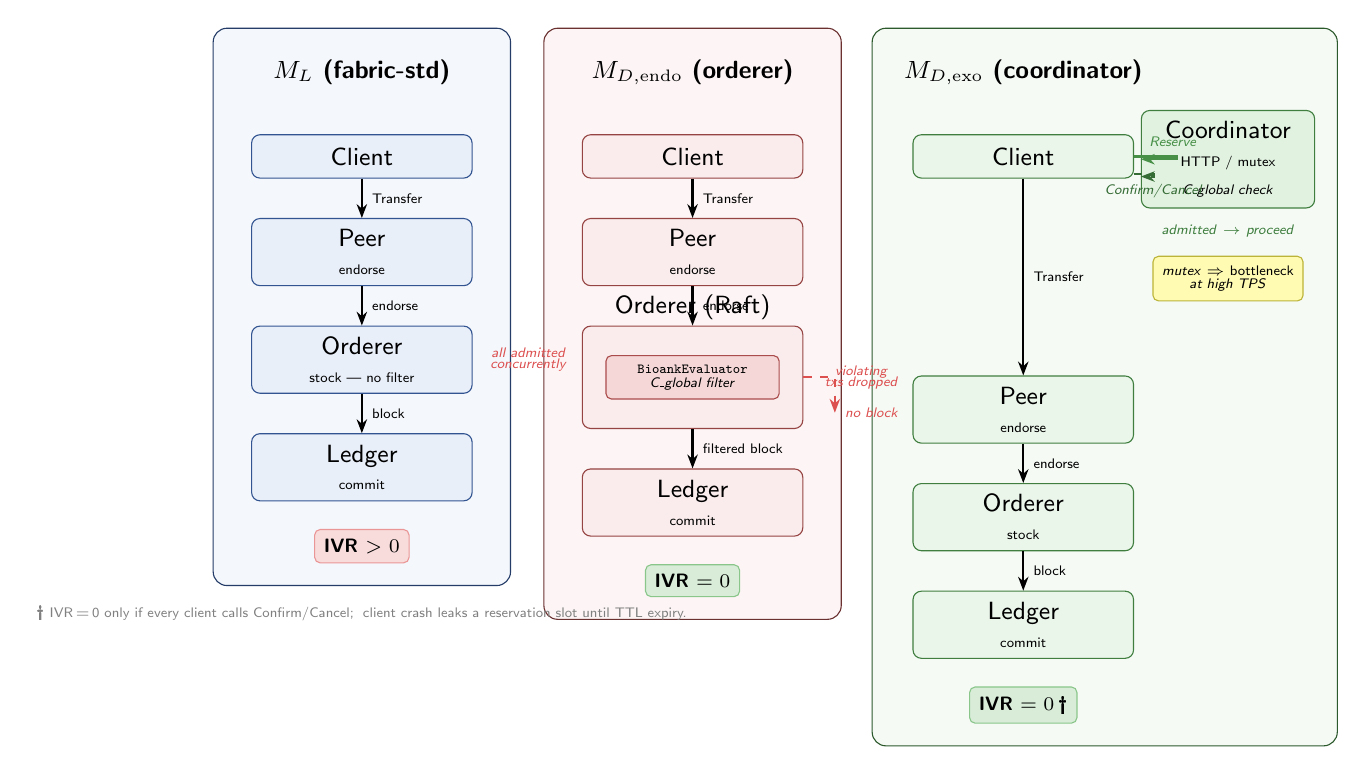
\begin{tikzpicture}[node distance=0.38cm]

% ── Column spacing ─────────────────────────────────────────────────────────────
\def\colA{0}
\def\colB{4.2}
\def\colC{8.4}

% ══════════════════════════════════════════════════════════
%  M_L column
% ══════════════════════════════════════════════════════════
\begin{scope}[xshift=\colA cm]
  % Header
  \node[colhead] (hML) at (1.6, 0)
    {$M_L$ \textbf{(fabric-std)}};

  % Nodes
  \node[box=cML, below=0.5cm of hML]     (cliML)  {Client};
  \node[box=cML, below=0.5cm of cliML]   (peerML) {Peer\\[-1pt]{\tiny endorse}};
  \node[box=cML, below=0.5cm of peerML]  (ordML)  {Orderer\\[-1pt]{\tiny stock — no filter}};
  \node[box=cML, below=0.5cm of ordML]   (ledML)  {Ledger\\[-1pt]{\tiny commit}};

  % Arrows
  \draw[arr] (cliML)  -- node[right, font=\tiny]{Transfer} (peerML);
  \draw[arr] (peerML) -- node[right, font=\tiny]{endorse}  (ordML);
  \draw[arr] (ordML)  -- node[right, font=\tiny]{block}    (ledML);

  % IVR badge
  \node[
    rectangle, rounded corners=2pt,
    fill=cReject!20, draw=cReject!60,
    font=\scriptsize\sffamily\bfseries,
    below=0.35cm of ledML,
  ] (ivrML) {IVR $> 0$};

  % Annotation: concurrent envelopes all admitted
  \node[
    font=\tiny\sffamily, text=cReject, align=center,
    right=0.1cm of ordML,
  ] {\textit{all admitted}\\[-2pt]\textit{concurrently}};

  % Column frame
  \begin{pgfonlayer}{background}
    \node[colframe=cML,
      fit=(hML)(cliML)(peerML)(ordML)(ledML)(ivrML),
    ] {};
  \end{pgfonlayer}
\end{scope}

% ══════════════════════════════════════════════════════════
%  M_D endogenous column
% ══════════════════════════════════════════════════════════
\begin{scope}[xshift=\colB cm]
  % Header
  \node[colhead] (hEndo) at (1.6, 0)
    {$M_{D,\mathrm{endo}}$ \textbf{(orderer)}};

  % Nodes
  \node[box=cEndo, below=0.5cm of hEndo]    (cliEndo)  {Client};
  \node[box=cEndo, below=0.5cm of cliEndo]  (peerEndo) {Peer\\[-1pt]{\tiny endorse}};

  % Orderer with evaluator sub-box
  \node[
    rectangle, rounded corners=3pt,
    draw=cEndo!70!black, fill=cEndo!12,
    minimum width=2.8cm, minimum height=1.3cm,
    below=0.5cm of peerEndo,
    font=\small\sffamily, align=center,
    inner sep=4pt,
  ] (ordEndo) {};
  \node[font=\small\sffamily, above=-0.05cm] at (ordEndo.north) {Orderer (Raft)};
  \node[
    rectangle, rounded corners=2pt,
    draw=cEndo!80!black, fill=cEndo!25,
    minimum width=2.2cm, minimum height=0.42cm,
    font=\tiny\sffamily, align=center,
  ] at (ordEndo.center) (eval) {\texttt{BioankEvaluator}\\[-1pt]\textit{C\_global filter}};

  \node[box=cEndo, below=0.5cm of ordEndo]  (ledEndo) {Ledger\\[-1pt]{\tiny commit}};

  % Drop path
  \node[
    font=\tiny\sffamily, text=cReject, align=center,
    right=0.15cm of ordEndo,
  ] (drop) {\textit{violating}\\[-2pt]\textit{txs dropped}};
  \draw[arrdashed, color=cReject]
    (ordEndo.east) -- ++(0.4,0) -- ++(0,-0.45)
    node[right, font=\tiny\sffamily, text=cReject]{\textit{no block}};

  % Main arrows
  \draw[arr] (cliEndo)  -- node[right, font=\tiny]{Transfer} (peerEndo);
  \draw[arr] (peerEndo) -- node[right, font=\tiny]{endorse}  (ordEndo);
  \draw[arr] (ordEndo)  -- node[right, font=\tiny]{filtered block} (ledEndo);

  % IVR badge
  \node[
    rectangle, rounded corners=2pt,
    fill=cCommit!20, draw=cCommit!60,
    font=\scriptsize\sffamily\bfseries,
    below=0.35cm of ledEndo,
  ] (ivrEndo) {IVR $= 0$};

  % Column frame
  \begin{pgfonlayer}{background}
    \node[colframe=cEndo,
      fit=(hEndo)(cliEndo)(peerEndo)(ordEndo)(ledEndo)(ivrEndo),
    ] {};
  \end{pgfonlayer}
\end{scope}

% ══════════════════════════════════════════════════════════
%  M_D exogenous column
% ══════════════════════════════════════════════════════════
\begin{scope}[xshift=\colC cm]
  % Header
  \node[colhead] (hExo) at (1.6, 0)
    {$M_{D,\mathrm{exo}}$ \textbf{(coordinator)}};

  % Coordinator (off to the right of main flow)
  \node[
    rectangle, rounded corners=3pt,
    draw=cExo!70!black, fill=cExo!18,
    minimum width=2.2cm, minimum height=0.9cm,
    font=\small\sffamily, align=center,
    inner sep=4pt,
  ] (coord) at (4.2, -1.1) {Coordinator\\[-1pt]{\tiny HTTP / mutex}\\[-1pt]{\tiny \textit{C\_global check}}};

  % Main flow nodes
  \node[box=cExo, below=0.5cm of hExo]    (cliExo)  {Client};
  \node[box=cExo, below=2.5cm of cliExo]  (peerExo) {Peer\\[-1pt]{\tiny endorse}};
  \node[box=cExo, below=0.5cm of peerExo] (ordExo)  {Orderer\\[-1pt]{\tiny stock}};
  \node[box=cExo, below=0.5cm of ordExo]  (ledExo)  {Ledger\\[-1pt]{\tiny commit}};

  % Reserve arrow (client → coordinator)
  \draw[arr, color=cExo!80!black]
    (cliExo.east) -- ++(0.55,0)
    node[above, font=\tiny\sffamily, pos=0.9]{\textit{Reserve}}
    |- (coord.west);

  % Confirm/Cancel arrow (client → coordinator)
  \draw[arrdashed, color=cExo!60!black]
    ($(cliExo.east)+(0.0,-0.22)$) -- ++(0.25,0)
    |- ($(coord.west)+(0,-0.22)$)
    node[below, font=\tiny\sffamily, pos=0.1]{\textit{Confirm/Cancel}};

  % Coordinator → admitted label
  \node[
    font=\tiny\sffamily, text=cExo!70!black,
    below=0.08cm of coord,
  ] {\textit{admitted} $\rightarrow$ \textit{proceed}};

  % Main arrows
  \draw[arr] (cliExo)  -- node[right, font=\tiny]{Transfer} (peerExo);
  \draw[arr] (peerExo) -- node[right, font=\tiny]{endorse}  (ordExo);
  \draw[arr] (ordExo)  -- node[right, font=\tiny]{block}    (ledExo);

  % Bottleneck annotation
  \node[
    rectangle, rounded corners=2pt,
    fill=yellow!30, draw=yellow!70!black,
    font=\tiny\sffamily, align=center,
    below=0.1cm of coord,
  ] at ($(coord.south)+(0,-0.5)$) {\textit{mutex} $\Rightarrow$ bottleneck\\[-1pt]\textit{at high TPS}};

  % IVR badge
  \node[
    rectangle, rounded corners=2pt,
    fill=cCommit!20, draw=cCommit!60,
    font=\scriptsize\sffamily\bfseries,
    below=0.35cm of ledExo,
  ] (ivrExo) {IVR $= 0$\,†};

  % Column frame
  \begin{pgfonlayer}{background}
    \node[colframe=cExo,
      fit=(hExo)(cliExo)(coord)(peerExo)(ordExo)(ledExo)(ivrExo),
    ] {};
  \end{pgfonlayer}
\end{scope}

% ── Global caption note ────────────────────────────────────────────────────────
\node[
  font=\tiny\sffamily, text=gray, align=left,
  below=1.2cm of ledML,
] {† IVR\,$=$\,0 only if every client calls Confirm/Cancel;\; client crash leaks a reservation slot until TTL expiry.};

\end{tikzpicture}
}% end \figArchitectures


% ==============================================================================
%  FIGURE 2 — Stable / speculative cache lifecycle
% ==============================================================================
\newcommand{\figCache}{%
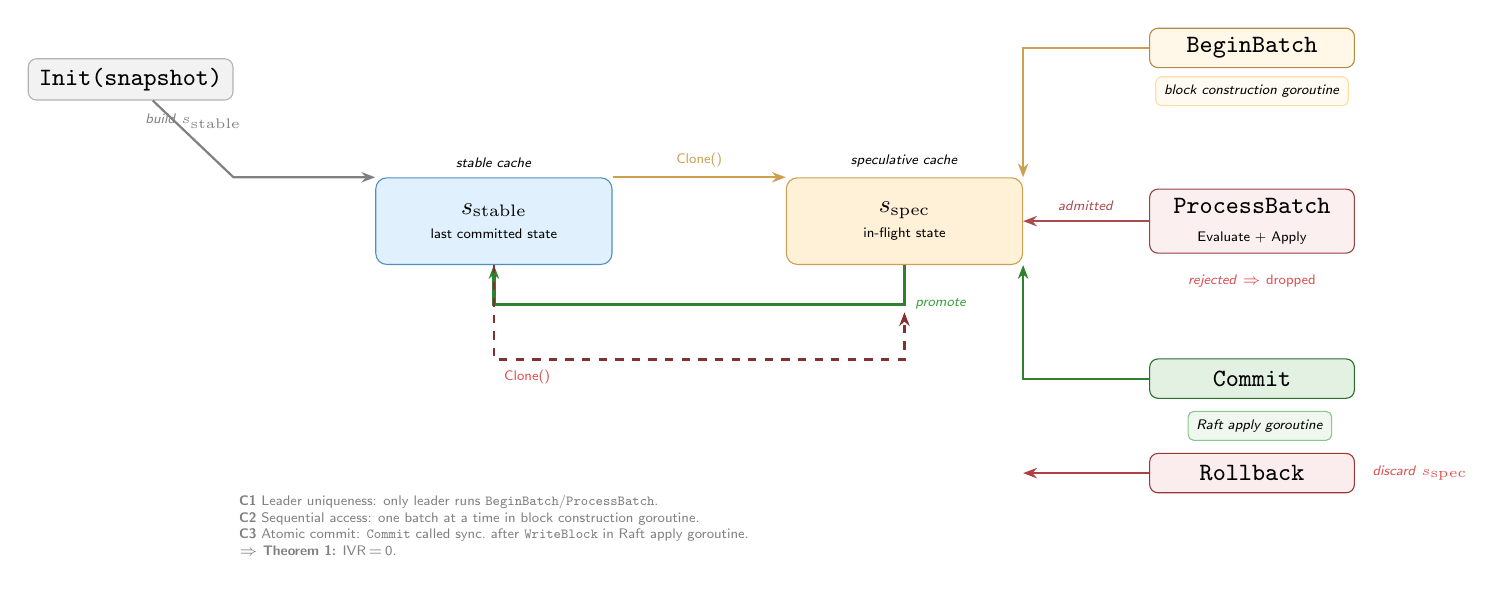
\begin{tikzpicture}[
  node distance=0.5cm and 1.8cm,
]

% ── Cache pair display ─────────────────────────────────────────────────────────
\def\cacheW{3.0cm}
\def\cacheH{1.1cm}

% Stable state box
\node[
  rectangle, rounded corners=4pt,
  draw=cStable!80!black, fill=cStable!20,
  minimum width=\cacheW, minimum height=\cacheH,
  font=\small\sffamily, align=center,
  label={[font=\tiny\sffamily]above:\textit{stable cache}},
] (stable) at (0,0) {$s_{\mathrm{stable}}$\\[-2pt]{\tiny last committed state}};

% Speculative state box
\node[
  rectangle, rounded corners=4pt,
  draw=cSpec!80!black, fill=cSpec!25,
  minimum width=\cacheW, minimum height=\cacheH,
  font=\small\sffamily, align=center,
  label={[font=\tiny\sffamily]above:\textit{speculative cache}},
  right=2.2cm of stable,
] (spec) {$s_{\mathrm{spec}}$\\[-2pt]{\tiny in-flight state}};

% ── Events on the left ─────────────────────────────────────────────────────────

% HandleChain / Init
\node[
  rectangle, rounded corners=3pt,
  draw=gray!60, fill=gray!10,
  minimum width=2.6cm, minimum height=0.5cm,
  font=\small\sffamily, align=center,
  left=1.8cm of stable, yshift=1.8cm,
] (init) {\texttt{Init(snapshot)}};

\draw[arr, gray]
  (init) -- node[above, font=\tiny\sffamily]{\textit{build} $s_{\mathrm{stable}}$}
  (stable.north -| init.east) -- (stable.north west);

% ── Events on the right (block construction loop) ─────────────────────────────

% BeginBatch
\node[
  rectangle, rounded corners=3pt,
  draw=cSpec!70!black, fill=cSpec!15,
  minimum width=2.6cm, minimum height=0.5cm,
  font=\small\sffamily, align=center,
  right=1.6cm of spec, yshift=2.2cm,
] (begin) {\texttt{BeginBatch}};

\draw[arr, color=cSpec!80!black]
  (stable.north east) --
  node[above, font=\tiny\sffamily]{Clone()} (spec.north west);
\draw[arr, color=cSpec!80!black]
  (begin) -- (spec.north east |- begin) -- (spec.north east);

% ProcessBatch — envelope loop
\node[
  rectangle, rounded corners=3pt,
  draw=cEndo!70!black, fill=cEndo!10,
  minimum width=2.6cm, minimum height=0.75cm,
  font=\small\sffamily, align=center,
  right=1.6cm of spec,
] (proc) {\texttt{ProcessBatch}\\[-1pt]{\tiny Evaluate + Apply}};

\draw[arr, color=cEndo!80!black]
  (proc.west) -- node[above, font=\tiny\sffamily]{\textit{admitted}} (spec.east);

% Rejected envelope
\node[
  font=\tiny\sffamily, text=cReject, align=center,
  below=0.15cm of proc,
] (rej) {\textit{rejected} $\Rightarrow$ dropped};

% Commit (success path)
\node[
  rectangle, rounded corners=3pt,
  draw=cCommit!70!black, fill=cCommit!15,
  minimum width=2.6cm, minimum height=0.5cm,
  font=\small\sffamily, align=center,
  right=1.6cm of spec, yshift=-2.0cm,
] (commit) {\texttt{Commit}};

\draw[arr, color=cCommit!80!black]
  (commit.west) -- (spec.east |- commit) -- (spec.south east);
\draw[arr, color=cCommit!80!black, very thick]
  (spec.south) -- ++(0,-0.5)
  node[right, font=\tiny\sffamily, text=cCommit]{\textit{promote}}
  -| (stable.south);

% Rollback (failure path)
\node[
  rectangle, rounded corners=3pt,
  draw=cReject!70!black, fill=cReject!10,
  minimum width=2.6cm, minimum height=0.5cm,
  font=\small\sffamily, align=center,
  right=1.6cm of spec, yshift=-3.2cm,
] (rollback) {\texttt{Rollback}};

\draw[arr, color=cReject!80!black]
  (rollback.west) -- (spec.east |- rollback);
\node[font=\tiny\sffamily, text=cReject, right=0.1cm of rollback]
  {\textit{discard} $s_{\mathrm{spec}}$};

% Stable re-clone on rollback
\draw[arrdashed, color=cReject!60!black]
  (stable.south) -- ++(0,-1.2)
  node[below right, font=\tiny\sffamily, text=cReject]{Clone()}
  -| ($(spec.south)+(0,-0.6)$);

% ── Goroutine labels ───────────────────────────────────────────────────────────
\node[
  rectangle, rounded corners=2pt,
  draw=cSpec!60, fill=cSpec!8,
  font=\tiny\sffamily, align=center, inner sep=3pt,
] at ($(begin)!0.5!(proc) + (0, 0.55)$) {\textit{block construction goroutine}};

\node[
  rectangle, rounded corners=2pt,
  draw=cCommit!60, fill=cCommit!8,
  font=\tiny\sffamily, align=center, inner sep=3pt,
] at ($(commit)!0.5!(rollback) + (0.1, 0)$) {\textit{Raft apply goroutine}};

% ── Invariant annotations ─────────────────────────────────────────────────────
\node[
  font=\tiny\sffamily, text=gray, align=left,
  below=2.8cm of stable,
] {
  \textbf{C1} Leader uniqueness: only leader runs \texttt{BeginBatch}/\texttt{ProcessBatch}.\\
  \textbf{C2} Sequential access: one batch at a time in block construction goroutine.\\
  \textbf{C3} Atomic commit: \texttt{Commit} called sync.\ after \texttt{WriteBlock} in Raft apply goroutine.\\
  $\Rightarrow$ \textbf{Theorem 1:} IVR\,$=$\,0.
};

\end{tikzpicture}
}% end \figCache


% ==============================================================================
%  Render both figures as standalone pages
% ==============================================================================
\begin{document}

% Page 1 — Architecture comparison
\figArchitectures

\newpage

% Page 2 — Cache lifecycle
\figCache

\end{document}
